%%%%%%%%%%%%%%%%%%%%%%%%%%%%%%%%%%%%%%%%%%%%%%%%%%%%%%%%%%%%%%%%%%%%%%%%%%%%%%%%%%%%%%
%%%%%%%%%%%%%%%%%%%%%%%%%          PRELIMINARY DESIGN        %%%%%%%%%%%%%%%%%%%%%%%%%
%%%%%%%%%%%%%%%%%%%%%%%%%%%%%%%%%%%%%%%%%%%%%%%%%%%%%%%%%%%%%%%%%%%%%%%%%%%%%%%%%%%%%%
\section{Preliminary Design}

%%%%%%%%%%%%%%%%%%%%%%%%%          DESIGN METHODOLOGY   
%%%%%%%%%%%%%%%%%%%%%%%%%%%%%%%%%%%%%%%%%%%%%%%%%%%%%%%%%%%%%%%%%%%%%%%%%%%%%%%%%%%%%%
\subsection{Design Methodology}

The preliminary configuration parameters of both aircraft were obtained through constraint analysis approach. This approach uses analytical equations which express aircraft power loading $\frac{P}{W}$, as a function of aircraft wing loading, $\frac{W}{S}$, and several other important parameters such as minimum drag coefficient, $C_{D0}$, induced drag constant $k$, propulsive efficiency $\eta_p$, climb rate $V_V$, climb velocity $V_{cmb}$, turn velocity $V_{trn}$, turn load factor $n$, and maximum lift coefficient  $C_{L_\text{max}}$. In addition to these parameters the aircraft power loading  is also affected by other various constraints, to name a few, laps that have to be flown, payload, and safety factors. The constraint analysis approach described in brief above was used for both aircraft. As there is a requirement that one aircraft should carry the other, either split in components or as a whole, the constraint analysis of both aircraft influence each other. 

\nomenclature{$C_{D0}$}{}%
\nomenclature{$k$}{}%
\nomenclature{$\eta_p$}{}%
\nomenclature{$V_V$}{}%
\nomenclature{$n$}{}%
\nomenclature{\frac{P}{W}}{}%
\nomenclature{$\frac{W}{S}$}{}%


%%%%%%%%
%%%%%%%%%%%%%%%%%%%%%%%%%          AIRFOIL SELECTION    
\subsubsection{Airfoil Selection}
Wings
In order to achieve the best performance for both aircraft, research had to be done to ensure the choice of  mission appropriate airfoils. Airfoil selection is one of the most crucial elements of an aircraft’s preliminary design since it impacts important aerodynamic aspects (e.g. drag, lift, stability). 
The selection of both aircraft’s airfoil was based on two factors, the competition’s missions and the difficulty of manufacturing. Just as it was mentioned at Part 1.3 of the report, the main factors that determine the required airfoil characteristics are the small take off distance, high cruise speed and high lift coefficient.

%%%%%%%%%%% SELECTION CRITERIA  
\paragraph{Selection criteria}
\begin{description}
    \item  [Maximum possible lift] at maximum efficiency. Both aircraft must complete missions that require the carrying of payload (Missions 2 and 3), which means the airfoils must be able to produce enough lift to easily carry the additional weight during the competition as well.
    \item [Climb rate and stall angle] must be high as well, since the takeoff distance is limited to 100 ft.
    \item [Power requirements] will rise once the first mission is completed. The extra weight that is added to the aircrafts in Mission 2 and 3 (i.e. transportation of small aircraft and the Gatorade bottle which must be carried by the production aircraft) increase the total weight, which increases the total lift, thrust and, consequently, the power required for cruising. The higher the lift the less the power needed for this purpose.
    \item[Drag coefficient]  must be have the minimum possible value, in order to maintain efficiency.
    \item[Pitching moment coefficient] must be kept to a minimum in order to reduce control surface requirements for the aircrafts’ stabilization which can lead to total weight reduction.
    \item[Thickness] plays a significant role as well. The airfoils cannot be too thin for manufacturing and fragility purposes and cannot also be too thick as it would cause an increase in profile drag.
\end{description}

%%%%%%%%%%% SELECTION PROCESS  
\paragraph{Selection process}

To begin with, various airfoils were researched using data from previous years, on-line resources and collected data from the University of Glasgow. Out of all the researched airfoils, the team gathered the few that could possibly fulfil the competition requirements and analyzed them using XFLR5.
 XFLR5 is a subsonic viscous two dimensional aerodynamics code that analyses and plots the characteristics of different airfoils, allowing their easy and fast comparison. All the airfoils were analyzed over a wide range of angle of attacks in order to determine the performance of each one of them for all of the predicted flight conditions. What is more, the specimens were tested at low Reynold’s numbers but the results were mainly focused on an estimated value of 250,000.
Eventually, the top two airfoils that met the design requirements, NACA 4412 and Clark Y, were compared. Their aerodynamic characteristics are shown at the graphs below. 
Firstly, Clark-Y has a lower lift coefficient for a given angle of attack (1.339 degrees) and a smaller stall angle than the ones of NACA 4412 (1.398 degrees). Secondly, the drag coefficient of the NACA airfoil is lower at low angles of attack which makes it even more suitable for cruising. Last but not least the moment coefficient of the NACA 4412 is lower that the  Clark-Y’s one, which fulfils another one of the previously mentioned requirements. 
It all boils down to the point that NACA 4412 is the most appropriate airfoil this year’s competition for both aircrafts, since their role is almost identical.


%%%%%%%%%%%%%%%%%%%%%%%%%          PARAMETER SELECTION  AND ESTIMATION
%%%%%%%%%%%%%%%%%%%%%%%%%%%%%%%%%%%%%%%%%%%%%%%%%%%%%%%%%%%%%%%%%%%%%%%%%%%%%%%%%%%%%%
\subsection{Parameter Selection and Estimation}

%%%%%%%%%%%%%%%%%%%%%%%%%          DRAG ESTIMATION  
\subsubsection{Drag Estimation}
Zero-lift drag buildup model from xx was used to determine drag component by component using 20 \si{\meter\per\second} reference airspeed. First, wetted areas of the exposed components were calculated and the fuselages of both aircraft were approximated as boxes that are reasonably bigger than the payload. The skin friction coefficients were then estimated, depending on the component location and the Reynolds number of the flow over the component. All components were assumed to have turbulent boundary layers, since they are either affected by the fuselage or are in the wake of the propeller.

%DRAG BUILD UP TABLES
\begin{table}[H]
\centering
    \begin{tabular}{@{}p{3cm}cccc@{}}
    \toprule
    \textbf{Component}       & \textbf{Wetted area (\si{\meter\squared})} & \textbf{Form factor} & \textbf{Equivalent flat plate area (\si{\meter\squared})} & \textbf{Parasitic drag coefficient} \\ \midrule
    
    \textbf{Wing}            & 0.4332               & 1.4556                 & 0.003695                                     & 0.0183                                \\
    
    \textbf{Horizontal tail} & 0.0831                    & 1.3447                 & 0.000138                                     & 0.0035                                  \\
    
    \textbf{Vertical tail}   & 0.0299                    & 1.3447                & 0.000019                                     & 0.0013                                 \\
    
    \textbf{Fuselage}        &    0.0671                  & 4.8462                   &   0.000577                                     &      0.0086                              \\
    \textbf{Total}    & -                    & -                    & 0.004429                                    & 0.0317                                 \\
    \textbf{Total including a factor of 1.06}    & -                    & -               & 0.004694                                          & 0.00336                                 \\
    \bottomrule
    \end{tabular}
\caption{PA drag buildup}
\label{tab:pa_drag_polar}
\end{table}
\begin{table}[H]
\centering

    \begin{tabular}{@{}lcccc@{}}
    \toprule
    \textbf{Component}       & \textbf{Wetted area (\si{\meter\squared})} & \textbf{Form factor} & \textbf{Equivalent parasitic drag area(\si{\meter\squared})} & \textbf{Parasite drag coefficient} \\ \midrule
    \textbf{Wing}            & 0.5870                    &    1.4556             & 0.005044                                      & -                                  \\
    \textbf{Horizontal tail} & -                    &    -             & -                                      & -                                  \\
    \textbf{Vertical tail}   & -                    &   -               & -                                      & -                                  \\
    \textbf{Fuselage}        &                      & -                    &                                        &                                    \\
    \textbf{Landing gear}    & -                    & -                    & -                                      & -                                  \\ \bottomrule
    \end{tabular}
\caption{MSA drag buildup}
\label{tab:msa_drag_polar}
\end{table}

Using the XFLR5 software, an average Oswald’s efficiency factor $e_{PA}$ for the production and $e_{MSA}$ for the manufacturing support aircraft was determined and drag polars for both were generated as shown in figures \ref{fig:pa_drag_polar} and \ref{fig:msa_drag_polar}.

%%%%% DRAG POLARS
\begin{figure}[H]
    \centering
    \includegraphics[width=9.72cm]{./preliminary_design/fig/dummy}
    \caption{PA drag polar}
    \label{fig:pa_drag_polar}
\end{figure}

\begin{figure}[H]
    \centering
    \includegraphics[width=9.72cm]{./preliminary_design/fig/dummy}
    \caption{MSA drag polar}
    \label{fig:msa_drag_polar}
\end{figure}

%%%%%%%%%%%%%%%%%%%%%%%%%          MASS ESTIMATION  
\subsubsection{Mass Estimation}
During the preliminary design stage both the wing and motor mass change due to changes in wing and power loadings. To account for these changes, wing density per area was first estimated based on previous reports describing similar aircraft configurations with similar aspect and taper ratios. This value was later refined with each iteration after the weight of the wing was estimated from the CAD model and the first prototype. As for motor mass a variety of motors were researched and their mass and power recorded. Form these values a motor mass versus power curve was generated as shown in figure \ref{fig: motor_mp}. Using this figure it was observed that in the low power range the mass-power relationship is linear. This relationship was used to estimate the preliminary motor mass for a particular aircraft power loading.

\begin{figure}[H]
    \centering
    \includegraphics[width=9.72cm]{./preliminary_design/fig/dummy}
    \caption{Motor mass-power plot}
    \label{fig: motor_mp}
\end{figure}


Mass values for other aircraft components were estimated in a similar manner. Existing components were analysed and their masses recorded after which an average value was calculated.

Similarly, battery mass also changes at different power loadings. This is due to the fact that at larger power loadings more powerful motors are required hence more powerful batteries. The battery mass estimation however was more difficult than the estimations for the mass of the wing and the motor. The aircraft performance was analysed during different sections of the mission - climb, turn, and cruise. From these analyses the peak power requirement was estimated. Based on this peak power value and battery cell specifications a relationship was developed which estimates the battery mass form the values of required power, battery C rating and chemical energy density.

\begin{equation}
    \text{Battery Mass} = \frac{\text{Maximum Power Requirement}}{\text{Battery C rating}\times\text{Battery energy density}}
\end{equation}

The mass estimations evaluated with the previously mentioned methods for both the PA and MSA are outlined in tables \ref{tab:pa_mass} and \ref{tab:msa_mass}. The aforementioned methods were used to estimate the mass of both aircraft at various power loadings.

\begin{table}[H]
\centering
    \begin{tabular}{@{}cc@{}}
    \toprule
    \textbf{Component}                          & \textbf{Mass (kg)} \\ \midrule
    \textbf{Servo}                              & -               \\
    \textbf{Receiver + Receiver battery + Fuse} & -               \\
    \textbf{ESC}                                & -               \\
    \textbf{Propeller}                          & -               \\
    \textbf{Motor}                              &                    \\
    \textbf{Wing}                               &                    \\
    \textbf{Battery}                            &                    \\
    \textbf{Fuselage}                           & -               \\
    \textbf{Landing gear}                       & -               \\ \bottomrule
    \end{tabular}
\caption{PA Mass Estimations}
\label{tab:pa_mass}
\end{table}
\begin{table}[H]
\centering
    \begin{tabular}{@{}cc@{}}
    \toprule
    \textbf{Component}                          & \textbf{Mass (kg)} \\ \midrule
    \textbf{Servo}                              & 0.03               \\
    \textbf{Receiver + Receiver battery + Fuse} & 0.06               \\
    \textbf{ESC}                                & 0.05               \\
    \textbf{Propeller}                          & 0.04               \\
    \textbf{Motor}                              &                    \\
    \textbf{Wing}                               &                    \\
    \textbf{Battery}                            &                    \\
    \textbf{Fuselage}                           & 0.2                \\
    \textbf{Landing gear}                       & 0.05               \\ \bottomrule
    \end{tabular}
\caption{MSA mass estimations}
\label{tab:msa_mass}
\end{table}


%%%%%%%%%%%%%%%%%%%%%%%%%          CONSTRAINT ANALYSIS   
%%%%%%%%%%%%%%%%%%%%%%%%%%%%%%%%%%%%%%%%%%%%%%%%%%%%%%%%%%%%%%%%%%%%%%%%%%%%%%%%%%%%%% 
\subsection{Constraint Analysis}
Several of the mission constraints for both aircraft include, but are not limited to 

\begin{enumerate}
    \item takeoff distance
    \item turn speed
    \item cruise speed
    \item climb speed
    \item rate of climb
\end{enumerate}

For the MSA an additional crucial mission constraint is payload dimensions and weight. Since the PA is going to be split in two subassemblies the former must be able to takeoff twice. As for the PA the main constraint is its dimensions and weight as it is the MSA payload. All of the above constraints are considered by the constraint analysis algorithm which determines the minimum aircraft mass at a particular $\frac{P}{W}$ and $\frac{W}{S}$ for which this is true.

%%%%%%%%%%% CONSTRAINT ANALYSIS ALGORITHM
\paragraph{Constraint Analysis Algorithm}

As discussed earlier the constraint analysis algorithm takes into account various constraints which are imposed by the mission that each aircraft must be able to complete. Therefore, each aircraft must satisfy a different set of constraints. By taking into account each constraint the algorithm iteratively calculates the power required for takeoff, turn, and climb at a particular wing loading. As the wing loading changes, other dependent parameters change accordingly. Other dependent parameters include wing area, wing mass, horizontal and vertical tail areas and masses in addition to motor mass. Accordingly, these changes influence the aircraft minimum drag coefficient, induced drag constant, all of which have an effect on the equations used in the constraint analysis. As a result these equations do not only depend upon on wing loading, but also on other parameters which are linked to wing loading. Consequently, an iterative approach is used by the algorithm in order to account for the previously mentioned dependencies. For each power and wing loading the algorithm iteratively changes the above mentioned parameter until the estimated empty mass of the aircraft converges. The result yielded by the algorithm is a family different curves for takeoff, turn and climb power loading which were plotted against the estimated empty mass of the aircraft.  A block diagram of the algorithm is shown below in figure \ref{fig:constraint_alg}.

\begin{figure}[H]
    \centering
    \includegraphics[width=9.72cm]{./preliminary_design/fig/dummy}
    \caption{Motor mass-power plot}
    \label{fig:constraint_alg}
\end{figure}


%%%%%%%%%%%%%%%%%%%%%%%%%          CONSTRAINT ANALYSIS   
%%%%%%%%%%%%%%%%%%%%%%%%%%%%%%%%%%%%%%%%%%%%%%%%%%%%%%%%%%%%%%%%%%%%%%%%%%%%%%%%%%%%%% 
\subsection{Mission Constraints}
%%%%%%%%
%%%%%%%%%%%%%%%%%%%%%%%%%          PA CONSTRAINT
\subsubsection{Production Aircraft}
The preliminary design of the production aircraft was carried out first due to the fact that the aircraft, when split in components, is the payload of the manufacturing support aircraft. This imposed a constraint on the production aircraft to be as small and light as possible. However making the aircraft smaller has an effect on other constraints which are discussed below.

\paragraph{Takeoff}
In case of the PA, takeoff is the most critical constraint. It dictates the minimum wing size with the selected maximum lift coefficient. The bigger the $C_{L_\text{max}}$ , the lower the stall speed and wing area, which would ultimately decrease the total mass.

\paragraph{Turn}
The aircraft is designed to fly at a design speed of 14 \si{\meter\per\second} during the turns. This speed is less than the design cruise speed of 20 \si{\meter\per\second} during the straight sections of the course. Having a lower turning speed reduces the load factor which in turn allows reduction wing strength and consequently mass.

\paragraph{Climb}

\paragraph{Constraint Analysis results}
\hfill

\begin{figure}[H]
    \centering
    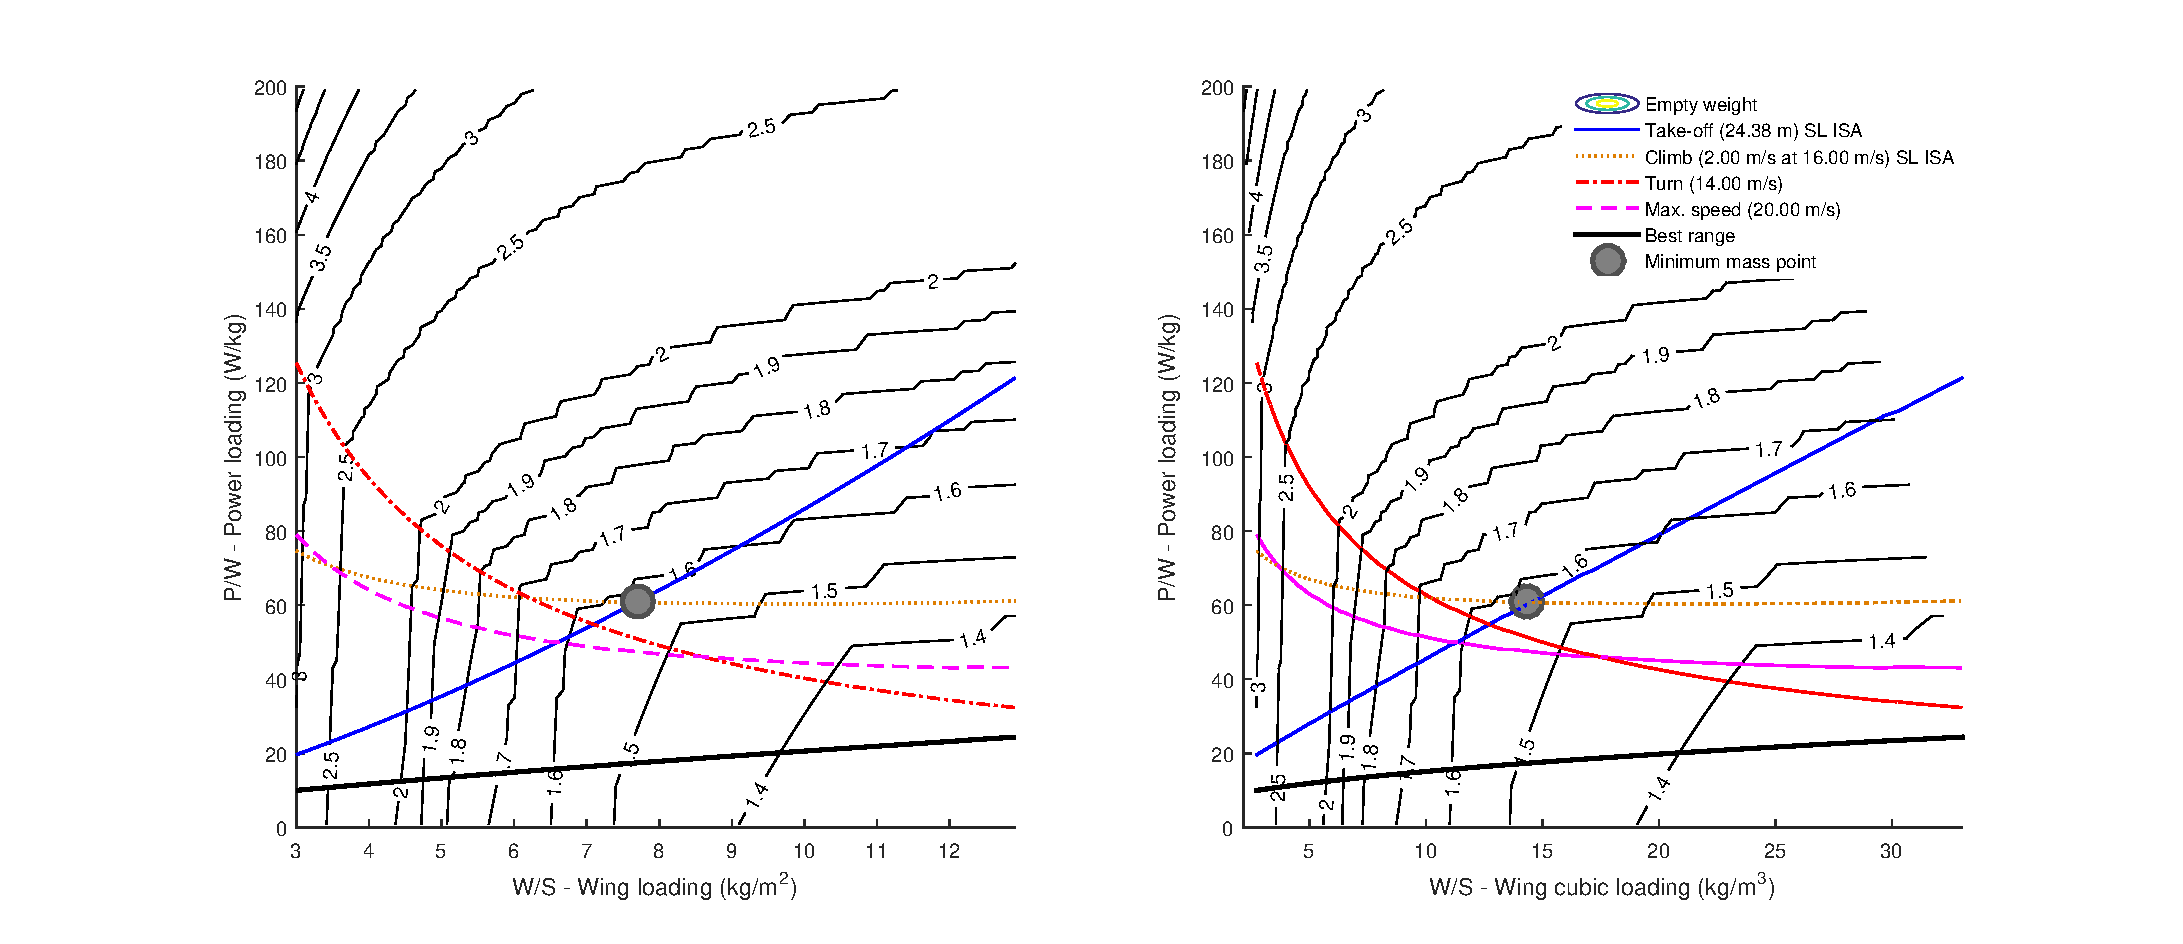
\includegraphics[width=\textwidth]{./preliminary_design/fig/pa_con}
    \caption{PA Constraint Analysis}
    \label{fig:pa_con}
\end{figure}

\begin{table}[H]
\centering

    \begin{tabular}{@{}ll@{}}
    \toprule
    \textbf{Safety factors and estimations}                                       & \textbf{Value} \\ \midrule
    \textbf{Takeoff distance safety factor}                                       & -          \\
    \textbf{Battery mass safety factor}                                           & -         \\
    \textbf{Estimated propulsive efficiency}                                      & -          \\
    \textbf{Estimated ground friction coefficient}                                & -        \\
    \textbf{Maximum achievable lift coefficient at reference airspeed (NACA4412)} & -         \\ \bottomrule
    \end{tabular}
\caption{Safety factors and key parameter estimations for PA}
\label{tab: pa_safety}
\end{table}
%%%%%%%%%%%%%%%%%%%%%%%%%          MSA CONSTRAINT
\subsubsection{Manufacturing Support Aircraft}

\paragraph{Takeoff}

\paragraph{Turn}

\paragraph{Climb}

\paragraph{Constraint Analysis results}
\begin{figure}[H]
    \centering
    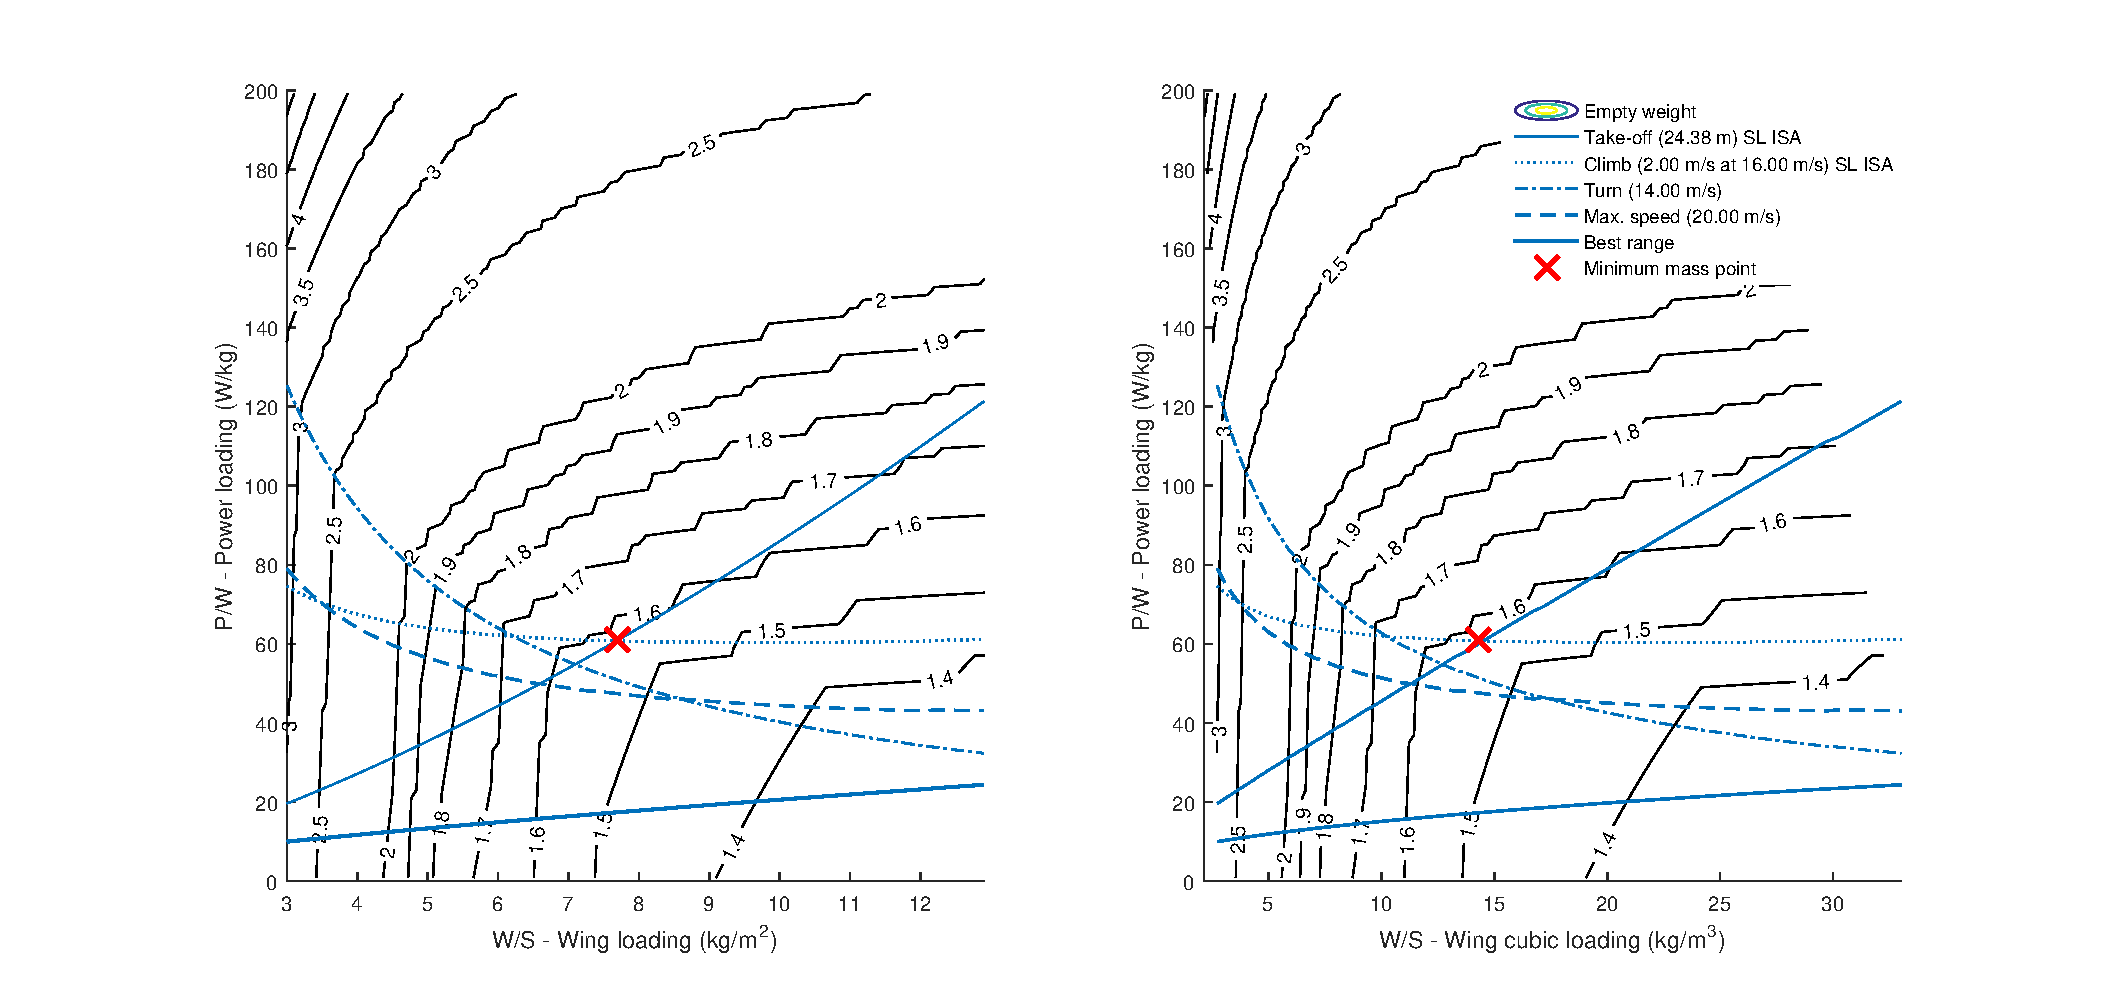
\includegraphics[width=\textwidth]{./preliminary_design/fig/msa_con}
    \caption{MSA drag polar}
    \label{fig:msa_con}
\end{figure}

\begin{table}[H]
\centering

    \begin{tabular}{@{}ll@{}}
    \toprule
    \textbf{Safety factors and estimations}                                       & \textbf{Value} \\ \midrule
    \textbf{Takeoff distance safety factor}                                       & -          \\
    \textbf{Battery mass safety factor}                                           & -         \\
    \textbf{Estimated propulsive efficiency}                                      & -          \\
    \textbf{Estimated ground friction coefficient}                                & -        \\
    \textbf{Maximum achievable lift coefficient at reference airspeed (NACA4412)} & -         \\ \bottomrule
    \end{tabular}
\caption{Safety factors and key parameter estimations for MSA}
\label{tab: msa_safety}
\end{table}


%%%%%%%%%%%%%%%%%%%%%%%%%          TRADEOFF STUDIES  
%%%%%%%%%%%%%%%%%%%%%%%%%%%%%%%%%%%%%%%%%%%%%%%%%%%%%%%%%%%%%%%%%%%%%%%%%%%%%%%%%%%%%% 
\subsection{Trade-off Studies}

In the constraint analysis figures \ref{fig:pa_con} and \ref{fig:msa_con} shown earlier, the minimum empty mass point which satisfies all constraints can be seen. For this point based on the input parameters provided to the algorithm, output parameters, both shown in the next section, such as wing area, horizontal tail area, empty mass, and more were calculated. However the output parameters at the minimum mass point for the production aircraft, though optimal, do not satisfy the previously imposed condition that this aircraft should be as small as possible in order to easily fit, when broken down in components in the manufacturing support aircraft. Due to this reason the parameters at the minimum mass point of the production aircraft were not used but instead, parameters at a desired wing loading  and power loading were selected. The new parameters ensured that the wing span and the horizontal tail span are small enough so that the production aircraft can fit into the fuselage of the manufacturing support aircraft. The reduction of the wing and horizontal tail span was achieved through increase in wing and power loading. In figure xx, showing the constraint analysis results for the production aircraft, marked with orange marker, is the selected point for specific wing and power loading. The drawback to reducing the span of the wing was that power had to be increased in order the takeoff constraint to be met. This issue arises due to the fact that wings with higher wing loading stall at higher speeds. For this reason below different values of wing loadings and their effects are discussed.

\begin{table}[H]
\centering
    \begin{tabular}{@{}lcc@{}}
    \toprule
                                        & \textbf{High Wing Loading} & \textbf{Low Wing Loading} \\ \midrule
    \textbf{Stall Speed}                & High                       & Low                       \\
    \textbf{Takeoff Distance}           & Long                       & Short                     \\
    \textbf{Maximum Lift to Drag Ratio} & High                       & Low                       \\
    \textbf{Gust Response}              & Good                       & Bad                       \\
    \textbf{Weight}                     & Low                        & High                      \\ \bottomrule
    \end{tabular}
\caption{Effect of different wing loadings on aircraft}
\label{tab: wingloading_var}
\end{table}

As a general rule????, loadings up to 3 \si{\kilo\gram\per\meter\squared} are for gentle flying, 3 \si{\kilo\gram\per\meter\squared} to 6 \si{\kilo\gram\per\meter\squared} for trainers and above 6 \si{\kilo\gram\per\meter\squared} for aerobatics. However, xxx suggests that wing cubic loading factor, defined as weight divided by the square root of the wing area , would be more appropriate to estimate the handling qualities for RC airplanes. Including the linear term (dividing by root of area, i.e. some reference length) in the wing loading equation introduces the airplane size as another factor. This makes it easier easier to categorize airplanes according to their ease of control. 

Wing cubic loading for the PA at the minimum mass point is 16.33 \si{\kilo\gram\per\meter\cubed} and at the selected specified wing and power loading point is 22.44 \si{\kilo\gram\per\meter\cubed}. According to xxx the aircraft would categorise as a expert sport for the former and as a expert only sport for the latter. It was decided that as long as the pilot has experience flying aircraft, handling qualities similar to a expert only sport aircraft are manageable, hence the selected wing and power loading point was selected. The selection of this point also satisfied the constraint of the production aircraft to be small.

The MSA has a wing cubic loading at the minimum mass point which varies from 9.99 \si{\kilo\gram\per\meter\cubed} when it is empty to 14.30 \si{\kilo\gram\per\meter\cubed} with full payload. Again according to xxx the aircraft would categorise as sport type a when empty and as advanced sport when flying with payload. As the the type of the production aircraft was selected to be expert only, the minimum mass point was selected.

\begin{table}[H]
\centering

    \begin{tabular}{@{}cCc@{}}
    \toprule
    \textbf{Level} & \textbf{Description}                                                                                                                                                  & \textbf{Average wing cubic load factor (kg/m3)} \\ \midrule
    \textbf{1}     & Includes mostly indoor type models and those that can be flown outside in very light winds, only level with no internal combustion powered planes                     & 2.39                                            \\
    \rowcolor[HTML]{EFEFEF} 
    \textbf{2}     & Includes mostly backyard type models that can be flown indoors in larger venues and outside in low wind conditions, includes a few internal combustion powered planes & 4.1                                             \\
    \textbf{3}     & Includes park flyers, sailplanes, biplanes, 3D planes                                                                                                                 & 5.99                                            \\
    \rowcolor[HTML]{EFEFEF} 
    \textbf{4}     & Includes sport types, biplanes, scale, a few 3D planes, pattern, largest level                                                                                        & 8.51                                            \\
    \textbf{5}     & Includes advanced sport types, sport scale and sport scale warbirds, some twins                                                                                       & 11.25                                           \\
    \rowcolor[HTML]{EFEFEF} 
    \textbf{6}     & Includes expert sport types, scale, scale warbirds, twins                                                                                                             & 14.31                                           \\
    \textbf{7}     & Includes planes for the expert flier only, twins and multi-motor, true scale, warbirds   
    \end{tabular}
\caption{RC aircraft general handling quality levels and respective wing cubic loadings}
\label{tab: wing_cubic}
\end{table}

\newpage 
%%%%%%%%%%%%%%%%%%%%%%%%%          ESTIMATED PARAMETERS 
%%%%%%%%%%%%%%%%%%%%%%%%%%%%%%%%%%%%%%%%%%%%%%%%%%%%%%%%%%%%%%%%%%%%%%%%%%%%%%%%%%%%%% 
\subsection{Estimated Parameters}
\begin{table}[H]
\centering
    \begin{tabular}{@{}Cl@{}}
    \toprule
    Important input parameters                                                                                    &        \\ \midrule
    Maximum lift coefficient                                                                                      & 1.5 -  \\
    \rowcolor[HTML]{EFEFEF} 
    Propulsive efficiency                                                                                         & 0.6 -  \\
    Wing aspect ratio                                                                                             & 5.5 -  \\
    \rowcolor[HTML]{EFEFEF} 
    Horizontal tail aspect ratio                                                                                  & 1.6 -  \\
    Vertical tail aspect ratio                                                                                    & 1 -    \\
    \rowcolor[HTML]{EFEFEF} 
    Vertical tail taper ratio                                                                                     & 0.5 -  \\
    Horizontal tail volume coefficient                                                                            & 0.6 -  \\
    \rowcolor[HTML]{EFEFEF} 
    Vertical tail volume coefficient                                                                              & 0.04 - \\
    Distance between the quarter chord position of the mean aerodynamic chord of the wing and the horizontal tail & 0.6 m  \\
    \rowcolor[HTML]{EFEFEF} 
    Distance between the quarter chord position of the mean aerodynamic chord of the wing and the vertical tail   & 0.6 m  \\ \bottomrule
    \end{tabular}
\caption{PA input parameters used for the constraint analysis algorithm}
\label{tab: pa_input}
\end{table}
\begin{savenotes}
\begin{table}[H]
\centering
    \begin{tabular}{@{}Cl@{}}
    \toprule
    \multicolumn{2}{l}{\textbf{Important output parameters for selected wing and power loading}} \\ \midrule
    \rowcolor[HTML]{EFEFEF} 
    \textbf{Wing loading}                                           & 10.1 \si{\kilo\gram\per\meter\squared}               \\
    \textbf{Wing area}                                              & 0.2024 \si{\meter\squared}                  \\
    \rowcolor[HTML]{EFEFEF} 
    \textbf{Wing span}                                              & 1.0552 \si{\meter}                   \\
    \textbf{Wing mean aerodynamic chord}                            & 0.1918 \si{\meter}                   \\
    \rowcolor[HTML]{EFEFEF} 
    \textbf{Horizontal tail area}                                   & 0.0388 \si{\meter\squared}                 \\
    \textbf{Horizontal tail span}                                   & 0.2493 \si{\meter}                    \\
    \rowcolor[HTML]{EFEFEF} 
    \textbf{Horizontal tail mean aerodynamic chord}                 & 0.1558 \si{\meter}                   \\
    \textbf{Vertical tail area}                                     & 0.0142 \si{\meter\squared}                  \\
    \rowcolor[HTML]{EFEFEF} 
    \textbf{Vertical tail span}                                     & 0.1193 \si{\meter} \\
    \textbf{Vertical tail mean aerodynamic chord}                   & 0.1237 \si{\meter}                    \\
    \rowcolor[HTML]{EFEFEF} 
    \textbf{Wing mass}                                              & 0.2020 \si{\kilo\gram}                 \\
    \textbf{Motor mass}                                             & 0.0626 \si{\kilo\gram}                  \\
    \rowcolor[HTML]{EFEFEF} 
    \textbf{Battery mass}                                           & 0.2700 \si{\kilo\gram}                  \\
    \textbf{Empty mass\footnote{Empty mass includes wing, motor and battery mass}}                                            & 1.1445 \si{\kilo\gram}                 \\
    \rowcolor[HTML]{EFEFEF} 
    \textbf{Mission mass}                                           & 2.0445 \si{\kilo\gram}                 \\
    \textbf{Takeoff power requirement}                              & 188.1000 \si{\watt}\\
    \rowcolor[HTML]{EFEFEF} 
    \textbf{Minimum drag coefficient}                               & 0.0293 -                   \\ \bottomrule
    \end{tabular}
\caption{Constraint analysis algorithm output parameters for PA}
\label{tab: pa_output}
\end{table}
\end{savenotes}
\newpage 
\begin{table}[H]
\centering

    \begin{tabular}{@{}Cl@{}}
    \toprule
    Important input parameters                                                                                    &        \\ \midrule
    Maximum lift coefficient                                                                                      & 1.5 -  \\
    \rowcolor[HTML]{EFEFEF} 
    Propulsive efficiency                                                                                         & 0.6 -  \\
    Wing aspect ratio                                                                                             & 8 -  \\
    \rowcolor[HTML]{EFEFEF} 
    Horizontal tail aspect ratio                                                                                  & 4 -  \\
    Vertical tail aspect ratio                                                                                    & 1 -    \\
    \rowcolor[HTML]{EFEFEF} 
    Vertical tail taper ratio                                                                                     & 0.5 -  \\
    Horizontal tail volume coefficient                                                                            & 1.2 -  \\
    \rowcolor[HTML]{EFEFEF} 
    Vertical tail volume coefficient                                                                              & 0.08 - \\
    Distance between the quarter chord position of the mean aerodynamic chord of the wing and the horizontal tail & 0.9 m  \\
    \rowcolor[HTML]{EFEFEF} 
    Distance between the quarter chord position of the mean aerodynamic chord of the wing and the vertical tail   & 0.9 m  \\ \bottomrule
    \end{tabular}
\caption{MSA input parameters used for the constraint analysis algorithm}
\label{tab: msa_input}
\end{table}
\begin{savenotes}
\begin{table}[H]
\centering
    \begin{tabular}{@{}Cl@{}}
    \toprule
    \multicolumn{2}{l}{\textbf{Important output parameters for selected wing and power loading}} \\ \midrule
    \rowcolor[HTML]{EFEFEF} 
    \textbf{Wing loading}                                           & 7.7 \si{\kilo\gram\per\meter\squared}               \\
    \textbf{Wing area}                                              & 0.2900 \si{\meter\squared}                  \\
    \rowcolor[HTML]{EFEFEF} 
    \textbf{Wing span}                                              & 1.5230 \si{\meter}                   \\
    \textbf{Wing mean aerodynamic chord}                            & 0.1904 \si{\meter}                   \\
    \rowcolor[HTML]{EFEFEF} 
    \textbf{Horizontal tail area}                                   & 0.0713 \si{\meter\squared}                 \\
    \textbf{Horizontal tail span}                                   & 0.5425 \si{\meter}                    \\
    \rowcolor[HTML]{EFEFEF} 
    \textbf{Horizontal tail mean aerodynamic chord}                 & 0.1356 \si{\meter}                   \\
    \textbf{Vertical tail area}                                     & 0.0380 \si{\meter\squared}                  \\
    \rowcolor[HTML]{EFEFEF} 
    \textbf{Vertical tail span}                                     & 0.1981 \si{\meter} \\
    \textbf{Vertical tail mean aerodynamic chord}                   & 0.2054 \si{\meter}                    \\
    \rowcolor[HTML]{EFEFEF} 
    \textbf{Wing mass}                                              & 0.2933 \si{\kilo\gram}                 \\
    \textbf{Motor mass}                                             & 0.0453 \si{\kilo\gram}                  \\
    \rowcolor[HTML]{EFEFEF} 
    \textbf{Battery mass}                                           & 0.2160 \si{\kilo\gram}                  \\
    \textbf{Empty mass\footnote{Empty mass includes wing, motor and battery mass}}                                            & 1.5646 \si{\kilo\gram}                 \\
    \rowcolor[HTML]{EFEFEF} 
    \textbf{Mission mass}                                           & 2.2366 \si{\kilo\gram}                 \\
    \textbf{Takeoff power requirement}                              & 136.1603 \si{\watt}\\
    \rowcolor[HTML]{EFEFEF} 
    \textbf{Minimum drag coefficient}                               & 0.0293                   \\ \bottomrule
    \end{tabular}

\caption{Constraint analysis algorithm output parameters for MSA}
\label{tab: msa_output}
\end{table}
\end{savenotes}

\newpage
%%%%%%%%%%%%%%%%%%%%%%%%%          PERFORMANCE
%%%%%%%%%%%%%%%%%%%%%%%%%%%%%%%%%%%%%%%%%%%%%%%%%%%%%%%%%%%%%%%%%%%%%%%%%%%%%%%%%%%%%% 
\subsection{Performance}

Both aircraft were designed to fly at a design speed of 20 \si{\meter\per\second} during the missions. The manufacturing support aircraft, when flying without a payload, in the first mission will experience more trim drag, however this will be compensated by higher dynamic thrust using a higher pitch propeller. An option to raise both ailerons to decrease the lift was discussed, but only after flight test will be decided whether it should be implemented.

\begin{table}[H]
\centering
    \begin{tabular}{@{}cccc@{}}
    \toprule
                                             & \textbf{Mission 1} & \textbf{Mission 2*} & \textbf{Mission 3} \\ \midrule
   \textbf{ Time, \si{\second} }                    & 129           & 103          & 153           \\
   \textbf{ $C_L$ (cruise)}                           & 0.2393             & 0.3205              & 0.4203             \\
   \textbf{ Stall speed, \si{\meter\per\second}}    & 7.99             & 9.24              & 10.58            \\
    \textbf{Takeoff speed, \si{\meter\per\second}}  & 9.59             & 11.09             & 12.70            \\
    \textbf{Best L/D speed, \si{\meter\per\second}} & 10.04            & 11.86             & 15.85            \\ \bottomrule
    \end{tabular}
\caption{Mission performance parameter estimates}
\label{tab: performance}
\end{table}

%%%%%%%%%%%%%%%%%%%%%%%%%          STABILITY AND TRIM
%%%%%%%%%%%%%%%%%%%%%%%%%%%%%%%%%%%%%%%%%%%%%%%%%%%%%%%%%%%%%%%%%%%%%%%%%%%%%%%%%%%%%% 
\subsection{Stability and Trim}

Aircraft static and dynamic stability are very important, especially for the manufacturing support aircraft which has to fly both empty and with payload.This results in changing center of gravity. Before the CAD models were developed an initial static stability analysis for both aircraft was carried out. Since one of the design parameters for the constraint analysis algorithm is the distance between the quarter chord position of the mean aerodynamic chord of the wing and the horizontal tail as well as the horizontal tail volume coefficient, another algorithm was developed which determines the stick-fixed neutral point of the wing-tail configurations for both aircraft. The algorithm not only determines the stick-fixed neutral points but also the required position of the center of gravity for a desired static margin and the required incidence angles of the wing and the tail such that the aircraft is trimmed at zero angle of attack with respect to the fuselage reference line and zero elevator deflection during cruise conditions. The algorithm was verified by the XFLR5 software. However the algorithm and the XFLR5 software did not take into account the effect of the fuselage on the stick-fixed neutral point. Therefore an initial conservative value of static margin for both aircraft was used as both fuselages will reduce it. A more precise refinement of the center of gravity position with respect to the neutral point will be carried out after flight testing. 

The benefit of performing these analyses is that if the center of gravity location for a particular static margin is known for both production and manufacturing support then it can be compared with the center of gravity from the CAD models and changes can be made if needed. An example of such change is when the CAD model of the production aircraft was developed and the actual center of gravity determined it was found out that the required center of gravity position and the actual of the manufacturing support aircraft were in considerable disagreement. A design change was made, the wing of the manufacturing support aircraft was moved slightly aft and the issue was resolved. After desired static stability results were achieved dynamic stability analysis were carried out with the XFLR5 software.


%%%%%%%%
%%%%%%%%%%%%%%%%%%%%%%%%%          STATIC STABILITY
\subsubsection{Static Stability}

Table xx shows the calculated location of the center of gravity for desired static margin for the manufacturing support aircraft. 


%%%%%%%%
%%%%%%%%%%%%%%%%%%%%%%%%%          DYNAMIC STABILITY
\subsubsection{Static Stability}


%%%%%%%%%%%%%%%%%%%%%%%%%          PROPULSION
%%%%%%%%%%%%%%%%%%%%%%%%%%%%%%%%%%%%%%%%%%%%%%%%%%%%%%%%%%%%%%%%%%%%%%%%%%%%%%%%%%%%%% 
\subsection{Propulsion}

%%%%%%%%
%%%%%%%%%%%%%%%%%%%%%%%%%          SELECTION
\subsubsection{Selection}

In order to design an optimal propulsion system for both aircraft, the following criteria was established:

\begin{itemize}
    \item Must be able to provide sufficient thrust for take-off.
    \item Weight of the whole propulsion system should be a minimum, especially batteries, to give the best performance and RAC.
    \item Propulsion system should be optimised for each mission. Especially important for the MSA, which must perform well in two missions with different requirements.
    \item Propellers must be within ground clearance limits. The PAS’s propeller diameter is constrained by the cross-sectional size of the MSA fuselage, due to the chosen configuration.
    \item Both aircraft must be able to achieve the design speed of 20\si{\meter\second}, for safe flight in gusty conditions common in Wichita.
\end{itemize}

Experience gained from the previous inaugural year’s entry supplied the team with valuable information. In 2015 our propulsion system had struggled during the most demanding mission, consequently  higher safety factors were used this year in addition to a more rigorous testing program. The Aeronaut CAMcarbon Power-Prop propellers were found to be exceptionally good as the larger diameter propellers produced comfortably more thrust than other propellers of the same size, so these would be predominantly tested where large diameter is required. RC Tiger Motors, T-Motors, were proven to be very reliable and efficient and were accordingly given extra consideration during the motor selection process.


%%%%%%%%
%%%%%%%%%%%%%%%%%%%%%%%%%         MOTOR AND PROPELLER SELECTION
\subsubsection{Selection}
\subsubsection{Motor and Propeller selection}

Based on the initial performance numbers and constraints, the type of motor and rough specifications were set. It was decided that a brushless out-runner motor would be used for both aircraft, due to their high efficiency, simplicity in using direct-drive and potential weight savings from not requiring a gearbox. 

For the Manufacturing Support Aircraft, a $K_V$ rating (no-load RPM per volt) of between 350 and 700, since there was little to no constraint on propeller size this would allow a large diameter, higher efficiency propeller to be used. The Production Aircraft’s propeller would be constrained to a maximum diameter of 10” (inches), so a $K_V$ in the range 800 to 1200 would be used. Propeller pitch needs to be large enough for the aircraft to fly at the design speed, the requirement will vary with motor, propeller and power supplied, but for the Manufacturing Support Aircraft will be greater than 10” and Production Aircraft greater than 6”. These, and the other requirements and constraints to be considered are shown in Table xx.

\nomenclature{$K_V$}{motor velocity constant}%

\begin{table}[H]
\centering

    \begin{tabular}{@{}cNNNNNNN@{}}
    \toprule
                                            & \textbf{Maximum Power Requirement(\si{\watt})} & \textbf{$K_v$ Range (rpm/V)} & \textbf{Maximum Propeller Diameter (inches)} & \textbf{Minimum Propeller Pitch (inches)} & \textbf{Minimum Take-off Speed (\si{\meter\per\second})} & \textbf{Design Speed (\si{\meter\per\second})} & \textbf{Maximum Ground Roll (\si{\meter})} \\ \midrule
    \textbf{PA}            & 188.1                                  & 800-1200                  & 10                                          & 6                                         & 12.7                                  & 20                          & 30.48 (100ft)                    \\
    \textbf{MSA} & 136.2                                  & 350-700                   & 15                                          & 10                                        & 11.09                                 & 20                          & 30.48 (100ft)                    \\ \bottomrule
    \end{tabular}
\caption{Propulsion requirements and constraints}
\label{tab: propulsion_requirement}
\end{table}